\documentclass{beamer}

\usepackage{amssymb}
\usepackage{epsfig,shadow}
\usepackage{beamerthemeshadow}

\beamertemplatetransparentcovereddynamic
\setbeamertemplate{navigation symbols}{}

%%%%%%%%%%%%%%
% Title page %
%%%%%%%%%%%%%%%%%%%%%%%%%%%%%%%%%%%%%%%%%%%%%%%%%%%%%%%%%%%%%%%%%%%%%%%%%%%%%%%

\title[OAR2]{
    OAR2\\
    An open source resource manager for large clusters
}
\author{
    LIG-ID\\
    Nicolas.Capit@imag.fr Olivier.Richard@imag.fr Yiannis.Georgiou@imag.fr
}

\institute{
    \begin{center}
        \includegraphics[scale=0.4]{src/img/oar_logo.png}
    \end{center}
    {\bf http://oar.imag.fr/}
}
\date{\today}

\begin{document}

\frame[plain]{\titlepage}

%%%%%%%%%%%%%%%%%%%%%
% Table of contents %
%%%%%%%%%%%%%%%%%%%%%%%%%%%%%%%%%%%%%%%%%%%%%%%%%%%%%%%%%%%%%%%%%%%%%%%%%%%%%%%

\frame{
    \frametitle{Part I: Production versions}
    \tableofcontents[pausesections,part=1]
}

\frame{
    \frametitle{Part II: Research}
    \tableofcontents[part=2]
}

%%%%%%%%%%%%%%
% First part %
%%%%%%%%%%%%%%%%%%%%%%%%%%%%%%%%%%%%%%%%%%%%%%%%%%%%%%%%%%%%%%%%%%%%%%%%%%%%%%%
\part{Production versions}
\frame{\partpage}

\section{Introduction}
    \subsection{Context}
        \frame{
            \frametitle{Context}
            \begin{itemize}
                \item TOTO
                \pause
                \item TITI
                \pause
                \item TITI
            \end{itemize}
        }

    \subsection{OAR2 key words}
        \frame{
            \frametitle{OAR2 key words}
            \begin{itemize}
                \item TOTO
            \end{itemize}
        }

    \subsection{Goals}
        \frame{
            \frametitle{OAR}
            \begin{itemize}
                \item TOTO2
            \end{itemize}
        }

\section{Strong concepts}
    \frame{
        \frametitle{OAR}
        \begin{center}
            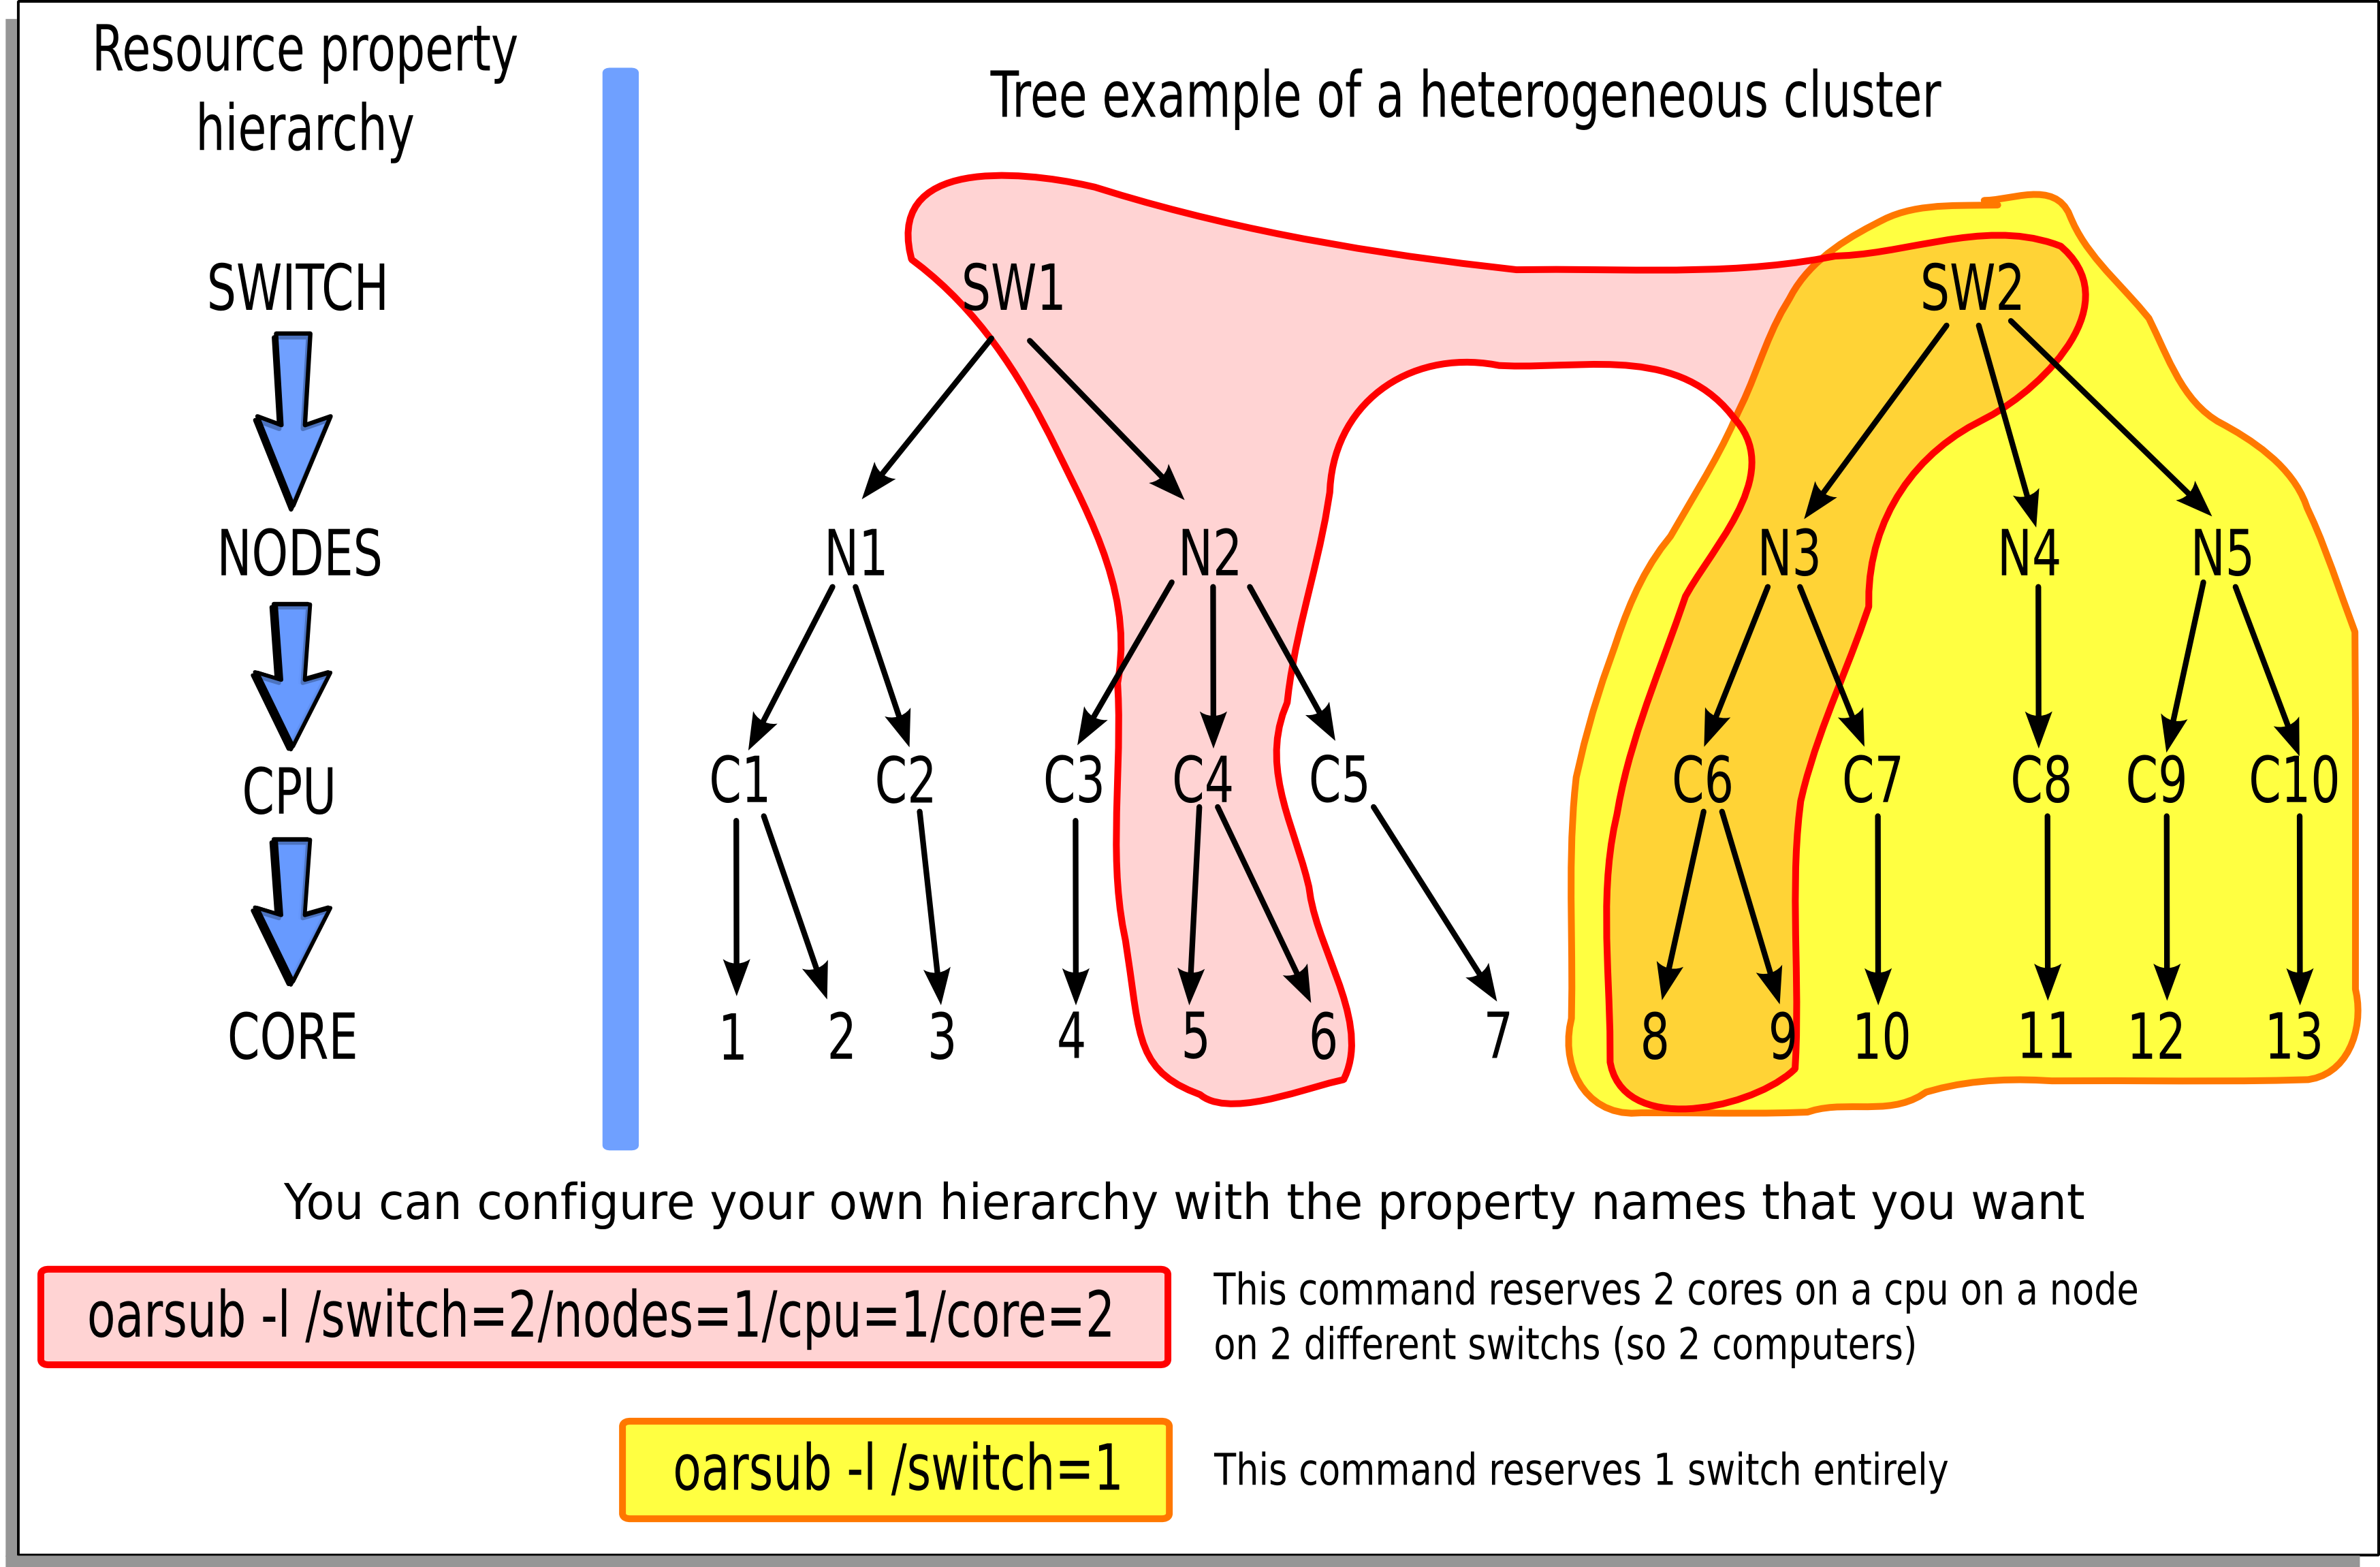
\includegraphics[height=40ex]{src/img/hierarchical_resources.png}
        \end{center}
    }

\section{Functionalities}
    \subsection{Administrator side}
        \frame{
            \frametitle{OAR}
            \begin{itemize}
                \item TOTO4
            \end{itemize}
        }

    \subsection{User side}
        \frame{
            \frametitle{OAR}
            \begin{itemize}
                \item TOTO4
            \end{itemize}
        }


    \subsection{Simple use cases}
        \frame{
            \frametitle{OAR}
            \begin{itemize}
                \item TOTO4
            \end{itemize}
        }

    \subsection{More complex use cases}
        \frame{
            \frametitle{OAR}
            \begin{itemize}
                \item TOTO4
            \end{itemize}
        }

\section{OAR2 in action}
    \frame{
        \frametitle{Part II: Research}
        \tableofcontents[pausesections,part=2]
    }

%%%%%%%%%%%%%%%
% Second part %
%%%%%%%%%%%%%%%%%%%%%%%%%%%%%%%%%%%%%%%%%%%%%%%%%%%%%%%%%%%%%%%%%%%%%%%%%%%%%%%
\part{Research}
\frame{\partpage}

\frame{
    \frametitle{Part II: Research}
    \tableofcontents[pausesections,part=2]
}


\section{YOPYOYPOP}
\frame{
    \frametitle{First slide}
    Yop
}

\section{YEPYEPEYEP}
\frame{
    \frametitle{Second slide}
    Yep
}

\end{document}

